\def\MWS{MathWebSearch\xspace}

A virtual research environment (VRE) has, as a foundation, a unified DKS\ednote{TW@MK: is this the tetrapod now} base and a joint user interface. 
The \pn approach is to create a mathematical VRE by integrating various pre-existing mathematical software systems. 
Furthermore, ``Computational notebooks'' (as reported on in~\cite{ODK-D4.2}) serve as an interface. 

Notebooks allow users to navigate the combined information space of all the underlying tools, systems and resources integrated into the VRE as one. 
However, they aggravate the already serious problem of finding anything. 
Thus, we decided to adapt the \MWS formula search engine to this joint user interface. 

\subsection{The \MWS Formula Search Engine}

\MWS is a web application that provides low-latency answers to full-text queries which consist of keywords and formulae.
We give only a brief overview of the pre-existing \MWS architecture here and refer the reader to~\cite{ProKoh:mwssofse12} and ~\cite{ODK-D6.1}. 
We furthermore describe our re-worked design in Section~\ref{sec:software:deployment} below.
In a nutshell, \MWS consists of a search web application (the \MWS daemon) that indexes formula harvests (essentially lists of content MathML formulae and URI references) and answers queries (Content MathML schemata with query variables).
Multiple domain-specific front-ends can talk to the \MWS daemon using an XML-based protocol, they transform the user's information into Content MathML queries. 

The \MWS system has been used to supply search instances on various corpora of mathematical documents, we describe two here, others can be seen on \url{http://search.mathweb.org}. 

\subsubsection{arXiv search}

Begun on August 14, 1991, created by Paul Ginsparg, the ``Cornell e-Print arXiv'' (\url{http://arXiv.org}) is a repository of scientific papers and electronic preprints in
fields of mathematics, computer science, physics, astronomy, biology and statistics or finance written in {\TeX/\LaTeX} for an optimized transfer over the internet and an easily rendered client-side.
In present the project is hosted by Cornell University and includes over a million articles and increases with around 8000 per month.

The KWARC group have converted by arXiv corpus into HTML5~\cite{StaKoh:tlcspx10} and harvested it for \MWS. The instance at \url{http://arxivsearch.mathweb.org}
indexes over 105\,000 math-heavy papers.
This subcorpus has also been used for the NTCIR Math Information Retrieval Challenges~\cite{AizKohOun:nmpto13,AizKohOunSch:nmto14,AizKohOunSch:nmto16}.

\subsubsection{zbMATH search}

Zentralblatt Math (zbMath) is a mathematical information service that curates a database of reviews and classifications (MSC, see~\cite{MSC2010}) for all articles in mathematics since the middle of the 19th century. The database currently contains 3.8 million reviews and grows at a rate of ca 120\,000 reviews per year.
The zbMATH portal at \url{https://zbmath.org/} offers a faceted search engine for reviews based on bibliographic metadata, MSC classification, and \emph{formulae}.
The latter is driven by \MWS. 

\subsection{Enabling Formula Search Deployments}\label{sec:software:deployment}

The previous \MWS deployments required a significant amount of application-specific code. 
This code was typically written by students, and as a result it was not of high quality. 
In particular, most code was too specialized to be re-usable. 

This made it impossible to directly use \MWS inside OpenDreamKit. 
To allow using \MWS flexibly, we needed to inject the system with a lot of software engineering. 
To achieve this, we developed new infrastructure on top of the core \MWS daemon. 
This works takes the form of several components, each of which can deployed independently using Docker (see also \WPref{component-architecture}).
The structure of our infrastructure can be seen in Figure~\ref{fig:mwsdeployment}, with new components in green. 

\begin{figure}[ht]
  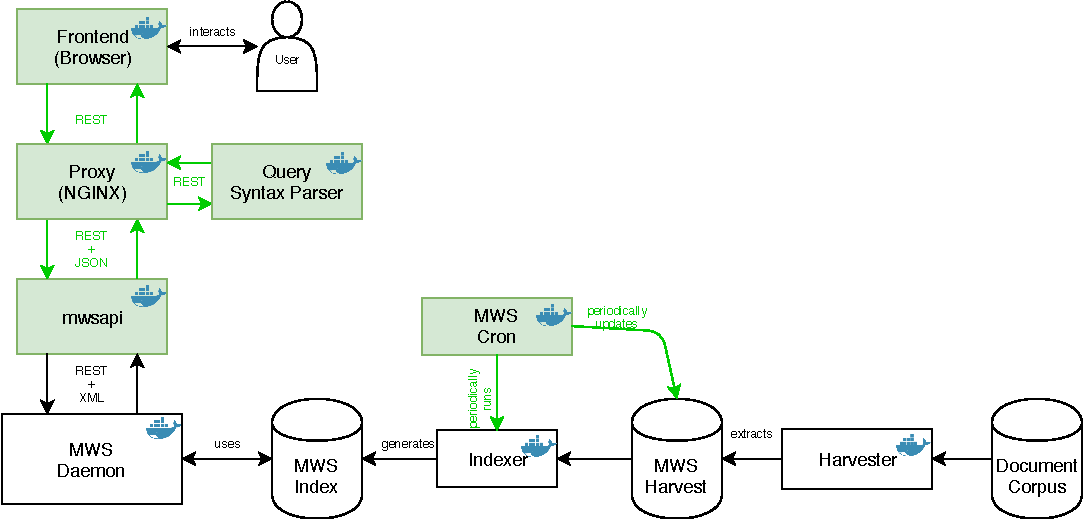
\includegraphics[width=0.8\textwidth]{mws_layout.pdf}
  \caption{Structure of our newly developed \MWS Deployment Infrastructure. Newly developed and updated components colored in green. }\label{fig:mwsdeployment}
\end{figure}

We describe the components of our infrastructure. 

\paragraph{The \MWS Daemon}
The central component is the \textit{\MWS daemon}, which can be found in the bottom left. 
As previously, it uses an \textit{Index} and exposes an XML-based API for queries. 
The only change we made to the core daemon is that it now exists inside a Docker Container at \footnote{\url{https://hub.docker.com/r/mathwebsearch/mathwebsearch/}}. 

\paragraph{The Harvesters and The Indexer}
As before, in order to generate an index from a set of documents we need two components. 
The indexer, as an application-independent component, has also been dockerized \footnote{\url{https://github.com/MathWebSearch/mws-indexer}}. 
First we extract a set of ContentMathML formulae using a corpus-specific \textit{Harvester} (bottom right). 
The generated \textit{Harvest} is then sent to the \textit{Indexer} (bottom center), which generates or updates the \textit{Index}. 

Additionally, we introduced a new scheduler component called \textit{MWS cron}. 
This periodically sends updated harvests to the \textit{indexer}, which then in turn updates the index. 
This process ensures that the Index remains up-to-date, and does not have to be re-generated manually. 
The source code of this component can be found at \footnote{\url{https://github.com/MathWebSearch/mws-cron}}. 

\paragraph{Frontend, mwsapi and the query syntax parser}

In order to process end user queries, we introduced several additional components.

The most important component of these is a new React-powered \textit{frontend}\footnote{\url{https://github.com/MathWebSearch/frontend}}, which runs inside the users' browser. 
It allows users to enter a formula search query, and view the results. 
The frontend contains corpus-specific branding and text, and is otherwise not corpus-specific. 
In particular the querying code which interacts with the backend components, does not require specialization. 

While the \MWS daemon only understands formulae in Content MathML, users often enter them using different representations, such as \LaTeX. 
For this purpose, the frontend allows entering queries in human-writable, corpus-specific syntax. 
In order to transform the user query into a system-understood query, we make use of a new component called the \textit{Query Syntax Parser}. 
For {\LaTeX} syntax this is achieved using {\LaTeX}ML along with a custom \MWS extension, but this component is fully interchangeable if the user desires other syntaxes. 

The frontend does not directly send MathML queries to the \textit{Daemon}.
Instead, it sends them to a thin API layer on top called \textit{mwsapi}. 
This layer forwards the queries to the daemon and, upon receiving a response, performs some post-processing. 
This process includes transforming substitutions returned by \MWS into a format that can be directly presented to the user by the frontend. 
The layer is written in go and doubles as api bindings to use MathWebSearch programatically in other applications. 
The source code and documentation are available on Github at \footnote{\url{https://github.com/MathWebSearch/mwsapi}}. 

As the frontend, the mwsapi server and the Query Syntax Presenter are all exposed to the end-user under the same url, a proxy delegating requests accordingly was also necessary. 
This is using an nginx server. 

\subsection{Building a Notebook Search}

Sage can produce \LaTeX\ formulae as output\ednote{TW@MK: Not sure how to describe this in more detail; should we ask Nicolas for this?}.
Using the newly developed infrastructure above, it was straightforward to apply \MWS and enable users to search for these formulae. 

Applying our infrastructure involved two steps, which we briefly describe below.

\paragraph{Harvesting Formulae}
To enable \MWS to search the formulae, we needed to build a harvester that extracted formulae from a notebook and as ContentMathML formulae. 
To achieve this, we converted each \LaTeX\ formula via LaTeXML and aggregated them inside an \MWS Harvest file. 
The script to achieve this can be found at \footnote{\url{https://github.com/OpenDreamKit/jupyter-notebook-harvester/blob/master/harvest}} and involved around 100 lines of straightforward Python script written in a few hours. 

To test our harvester, we decided to make use of Sage Jupyter Notebooks found on GitHub. 
We implemented a second Python script which used the GitHub API to download all matching files and then apply our harvester to them. 
This process resulted in an \MWS Harvest of $0$ documents, containing $0$ formulae\ednote{TW: Update numbers}.

\paragraph{Query Syntax Parser}

To enable users to search the formulae in an appropriate syntax, a query syntax parser was required. 
However, as Sage produces \LaTeX\ formulae, we can re-use the {\LaTeX}ML query syntax parser for this purpose. 

\paragraph{Deploying the system}

\begin{figure}[ht]
  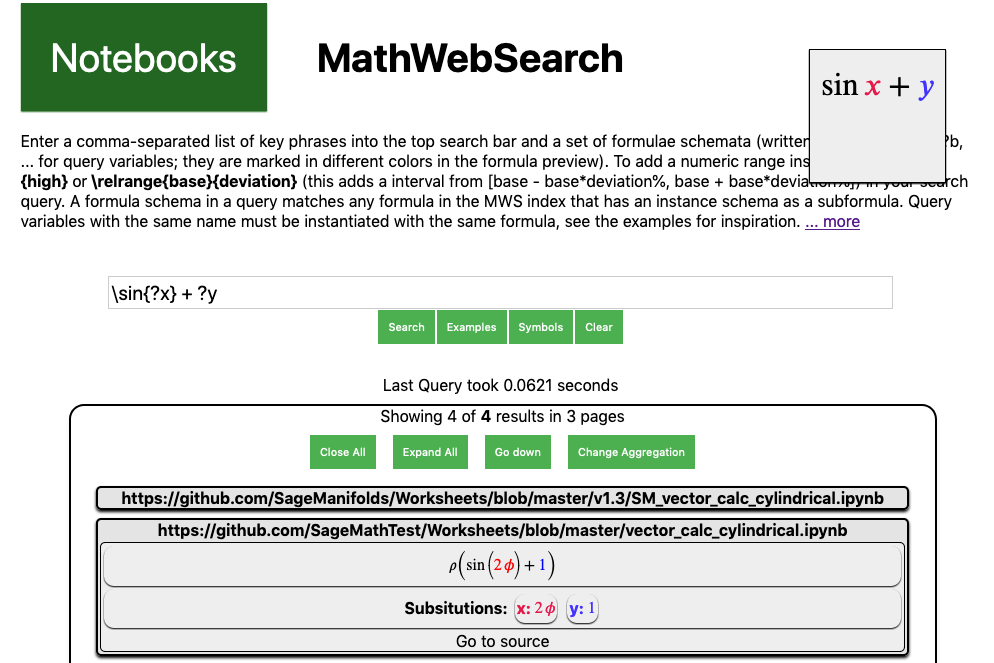
\includegraphics[width=\textwidth]{mwsnotebookfront.png}
  \caption{The deployed Jupyter Notebook Search Frontend}\label{fig:mwsnotebookfront}
\end{figure}

The third and final step involved deploying the system.
This required minor customization in the branding of the frontend. 
The user interface is deployed at \url{https://jupytersearch.mathweb.org} and can be seen in Figure~\ref{fig:mwsnotebookfront}.

In addition the notebook search, we have also exercised a similar progress for NLab. 
\ednote{TW@MK: Do I have to explain what nlab is or can I assume the readers know?}
Similar to notebooks, NLab also contains formulae in \LaTeX\ syntax, enabling us to largely re-use all components we had created previously.
The NLab Harvester can be found at \footnote{\url{https://github.com/MathWebSearch/nlab_harvester}}, and the corresponding frontend at \url{https://nlabsearch.mathweb.org}. 

%%% Local Variables:
%%% mode: latex
%%% mode: visual-line
%%% fill-column: 5000
%%% TeX-master: "report"
%%% End:

%  LocalWords:  ednote textbf fig:mwsdeployment includegraphics textwidth mws_layout.pdf textit mwsapi specialization nginx Jupyter customized evalutation temasearch xspace newpart standardized ProKoh:mwssofse12 subsubsection Ginsparg optimized StaKoh:tlcspx10 AizKohOun:nmpto13,AizKohOunSch:nmto14,AizKohOunSch:nmto16 zbMATH emph specialized WPref colored dockerized customization NLab oldpart mwsnotebookfront.png fig:mwsnotebookfront
